\section{Introduction}
\label{sec:intro}
%
Data visualization is one of the most common tools for identifying trends and finding anomalies in Big Data. 
%
However, with high-dimensional datasets, identifying visualizations that effectively present interesting variations or patterns in the data is a not a trivial task: analysts typically build a large number of visualizations optimizing for a range of visualization types, appealing features, and more before arriving at one that shows something valuable. 
%

For datasets with large number of dimensions, it is extremely exhaustive for analysts to manually study all the dimensions; hence, interactive data visualization needs to be boosted with automated visualizations recommendation techniques.
%
Interactive visualization analytics tools such as Tableau, ShowMe, and Fusion Tables \cite{DBLP:conf/sigmod/GonzalezHJLMSSG10,DBLP:journals/tvcg/MackinlayHS07,Stolte:2000:PSQ:857190.857686} provide some features for automatically recommending the best visualization for a dataset. However, these features are restricted to a set of aesthetic rules (e.g., color, fonts, styles, ... etc) that guide which visualization is most appropriate.
% Ibrahim
%provide users with visualizations built from structured, weakly structured and unstructured data.
%
%While they are successful in building meaningful visualizations, they lack the ability to automatically recommend visualizations that are considered interesting and rely on the analysts' own judgments.
%
%
%partially provide some features for automatically recommending the best visualization for a dataset. 
%
%these features are restricted to a set of aesthetic rules that guide which 
%visualization is most appropriate. 
%

Profiler \cite{kandel2012profiler}, is another visualization tool which explores all data space to detect anomalies in data and recommends the best binning for the horizontal $x$ axis of a visualization. It decides which granularity is appropriate to bin on to depict the most interesting relationships among data.
%
%are limited only to determine the best binning for the for the horizontal axis. 
%
%detect anomalies in data
%
%are exploring all data and the visualizations space 
%to detects anomalies in data and provide some visualization recommendation functionality. Although, those tools
%are limited only to determine . 
%
%Other tools such as Profiler \cite{kandel2012profiler} are exploring all data and the visualizations space 
%to 
%
Profiler \cite{kandel2012profiler} maintains a data cube in memory and uses it to support rapid user interactions.
%
While this approach is possible when the dimensionality and cardinality are small, it cannot be used with large tables and ad-hoc queries with high dimensional data, which is the norm of scientific databases.
%

In the bio-medical data analysis domain, INVISQUE \cite{Wong2011,DBLP:conf/chi/WongCKRX11} was proposed as a visual sense-making system to support information analysis for medical diagnosis. 
%
INVISQUE illustrates the similarity between the information analysis during intelligence analysis and medical diagnosis based on a Sense-Making Loop and a Data-Frame model.
%
To overcome the challenges of exploring high-dimensional patients data,  SubVIS \cite{Hund2016} was recently proposed as a visualization tool to interactively explore bio-medical data by utilizing subspace analysis algorithms to cluster data into sub clusters and show the relationships that exist among them.
%
\begin{figure}[t]
  \centering
    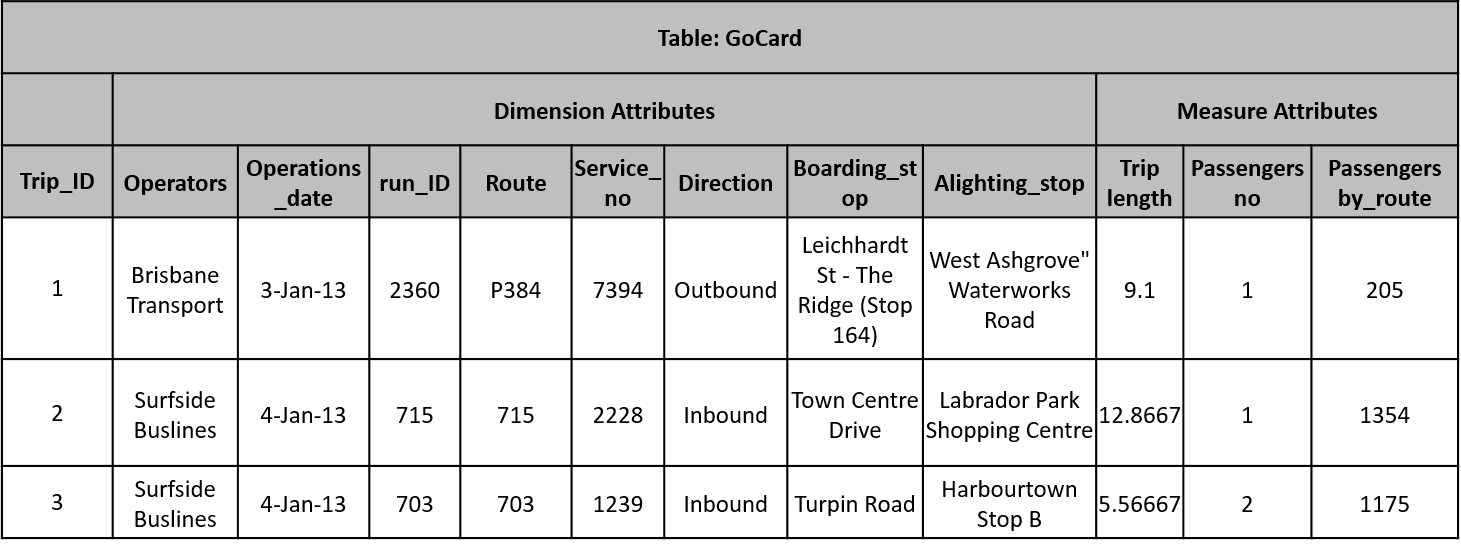
\includegraphics[width=\textwidth]{gocard_schemaandsample.png}
    \caption{Snippet from the GoCard relational database schema with a representative sample. Each row represents one trip with a bus, a ferry or a train with 12 dimensions describing the details of that trip. 
		%
		The database's dimensions are classified into two: dimension attributes and measure attributes, in order to generate meaningful 2-dimensional visualizations, e.g., bar charts.
		}
    \label{fig:gocard_schemaandsample}
\end{figure}

Another example of tools that recommend visualizations is VizDeck \cite{DBLP:conf/sigmod/KeyHPA12}. 
%
VizDeck recommends visualizations based on the statistical properties of small datasets and adopts a card game metaphor 
to help organize the recommended visualizations into interactive visual dashboard.
%
%VizDeck does not discuss techniques to efficiently generate these visualizations.
%

For large scale datasets, SeeDB \cite{DBLP:journals/pvldb/VartakMPP14} was proposed to automatically recommend interesting visualizations based on distance metrics which compute deviations among the probability distributions of the 
visualizations. 
%
SeeDB presents different levels of optimizations to decrease the latency and maintain the quality of visualizations such as sharing computations and combined query executions.
%

Although, these analytic tools present various approaches and measures to asses the interestingness of data, they still have to explore all possible visualizations to recommend a subset of interesting visualizations.
%
Exploring the entire data space and all visualizations is almost impossible with the limited time and resources, especially when data is growing in both the dimensionality and cardinality.
% 
As a result, shifting from static analytics to realtime analytics is essential because of the rapid data accumulation when compared with a constant human cognitive capacity. 
%
Indeed this is a challenging problem.
%
An interactive visualizations recommendation tool needs to explore the data space intelligently by discounting unnecessary visualizations and recommend only the essential ones while preserving the quality of the results.
%
%
%
%
%
%
%
%
%\blue{introduce GoCard data and example.}
%
%
%
%

The following example illustrates the need for an automatic visualizations technique to identify interesting visualizations from a real, large and structured database called GoCard which represents trips details of the public transportation system of the Brisbane city in Australia.
%
Figure \ref{fig:gocard_schemaandsample} shows a snippet of the GoCard database schema and a small sample from the database out of the 4.4 million tuples.
%
Each tuple is a record that represents a trip using either a bus, a ferry or a train, with 12 dimensions describing that trip with more details.
%
%
%
\eat{
\begin{table}[t]
\centering
\caption{Results of query $Q_1$ and $Q_r$: Average trips length in minutes by boarding stop of the view $Q_1$ and the reference view $Q_r$ result into high utility value, i.e., high interestingness. }{
%\begin{center}
\begin{tabular}{|c|c|c|} \hline
& \multicolumn{2}{|c|}{\textbf{Trip Length (min)}}  \\ \hline
\textbf{Boarding Stop} & $Q_1$ & $Q_r$ \\ \hline
	Macarthur Ave : Northshore Hamilton & 74.85 &  34.12\\ \hline
Apollo Ferry Terminal & 70.27 & 26.79\\ \hline
Bretts Wharf Ferry Terminal & 67.01 & 26.24 \\ \hline
Griffith University station  & 61.83 & 11.40\\ \hline
Bulimba Ferry Terminal  & 60.13 & 14.81\\ \hline
%King George Square Station 1A  & 929.3499756 \\ \hline
\end{tabular}}
%\end{center}
\label{tab:q1_result}
\end{table}
}
%
%
%
%
%
\begin{figure}[t]
  \begin{subfigure}[b]{0.45\textwidth}
    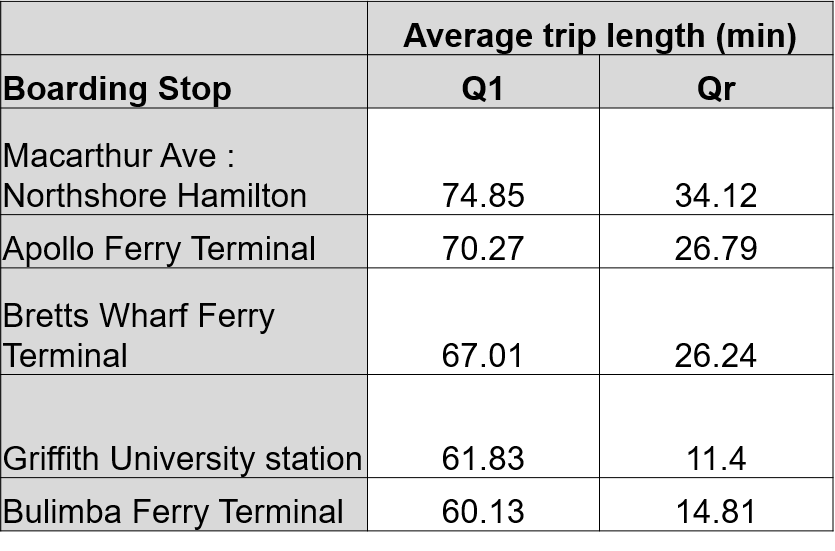
\includegraphics[width=\textwidth]{table_gocard_ex.png}
    \caption{Sample results of query $Q_1$ and $Q_r$}
       \label{fig:table_gocard_ex}
  \end{subfigure}
	\begin{subfigure}[b]{0.45\textwidth}
    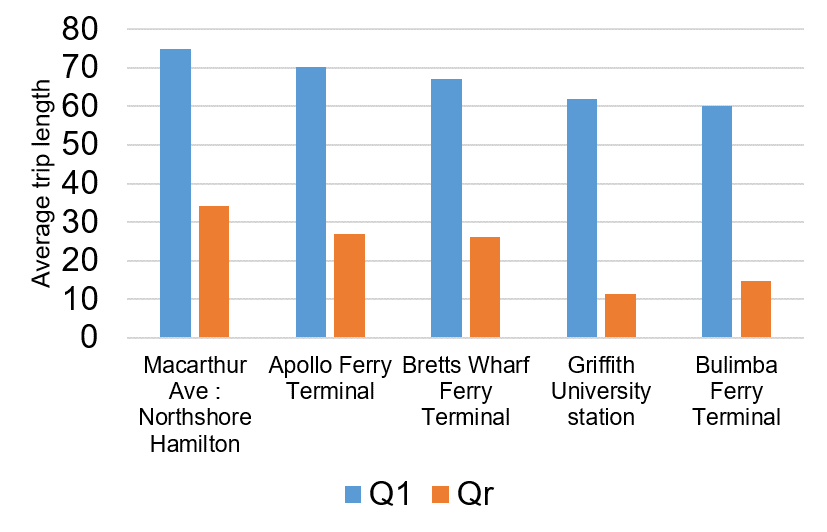
\includegraphics[width=\textwidth]{chart_gocard_ex.png}
    \caption{2-D bar chart for query $Q_1$ and $Q_r$}
       \label{fig:chart_gocard_ex}
  \end{subfigure}
  %
  \caption{Average trips length in minutes by boarding stop of $Q_1$ and the reference $Q_r$ result into high utility value, i.e., high \emph{interestingness}}
\end{figure}
%
\begin{example}
\label{ex:gocard}
%
Consider a transportation analytic team that is undertaking a study for a particular alighting stop: \emph{University of Queensland} (UQ).
%
This stop has received a lot of passengers’ complaints due to poor performance, hence, it is being investigated by the team.
%
Suppose that the team uses the GoCard database to generate 2-dimensional visualizations (e.g., bar charts) which summarize all recorded trips using different dimensions, then search for the ones that appear to explain the increase in received complaints. 
%
To accomplish that, an analyst would begin by using a program's GUI or a custom 
query language to execute the equivalent of the following SQL query and pull all data from the database for the alighting stop UQ:
%
\begin{center}
\texttt{$Q$ = SELECT * FROM GoCard \\ WHERE alighting stop ="University of Queensland";}
\end{center}
%
Next, the analyst would use an interactive GUI interface to generate all possible visualizations of the query result.
%
%
%containing metrics such as trip length and daily passengers for each route. 
%
%Also, it has a large set of dimension attributes containing information such as operators, service number, operations date, day, direction, boarding stop, alighting stop, etc, as shown earlier in Table \ref{tab:gocard_database}.
%
%Given the large size of the database (millions of records), an analyst will overwhelmingly 
%use a collection of visualization programs to gather insights into the behavior of the alighting stop UQ.
%
%In a typical analysis workflow, 
%
%
For instance, the analyst may visualize average trip length grouped by route, total daily passengers grouped by direction, maximum trip length by boarding stop, and so on. 
%
Hence, the analyst would manually study all these visualizations to find interesting insight or visualizations that might explain the  reason behind the increase of complaints.
%
Indeed, exploring and studying all visualizations is challenging especially for high dimensional datasets.  %impossible.
%
Hence, an automatic visualization recommendation technique should show the analyst the most interesting visualization based on the alighting stop UQ.
%
%Under the hood, these visualization operations are essentially queries to the underlying database and subsequent graphing of the results. 
%

Consider the visualization for the average trip length by boarding stop: it is generated by running an operation equivalent to the following SQL query:
%
\begin{center} 
\texttt{ $Q_1$ = SELECT boarding stop, AVG(trip length)  FROM GoCard 
\\ WHERE alighting stop ="University of Queensland"  GROUP BY boarding stop; } 
\end{center}
%
Figure \ref{fig:q1_vis} shows the visualization of $Q_1$'s result.
%
Consequently, the visualization in Figure \ref{fig:q1_vis} happened to be the most interesting visualization.
%
The reason is, when $Q_1$'s result is compared with entire data, it depicts long average trip length in some boarding stops which travels towards UQ that are significantly different from the equivalent average of the trip lengths (equals 17.6 minutes) in the entire dataset.
%
Specifically, $Q_1$'s result is compared against the following reference query $Q_r$:
%
\begin{center} 
\texttt{ $Q_r$ = SELECT boarding stop, AVG(trip length)  FROM GoCard 
\\  GROUP BY boarding stop; } 
\end{center}
%
The Figures \ref{fig:table_gocard_ex} and \ref{fig:chart_gocard_ex} show a sample results of $Q_1$ and $Q_r$.
%
\qed
\end{example}
%
%
%
%
%
%
%
%
\begin{figure}[t] 
	\centering
	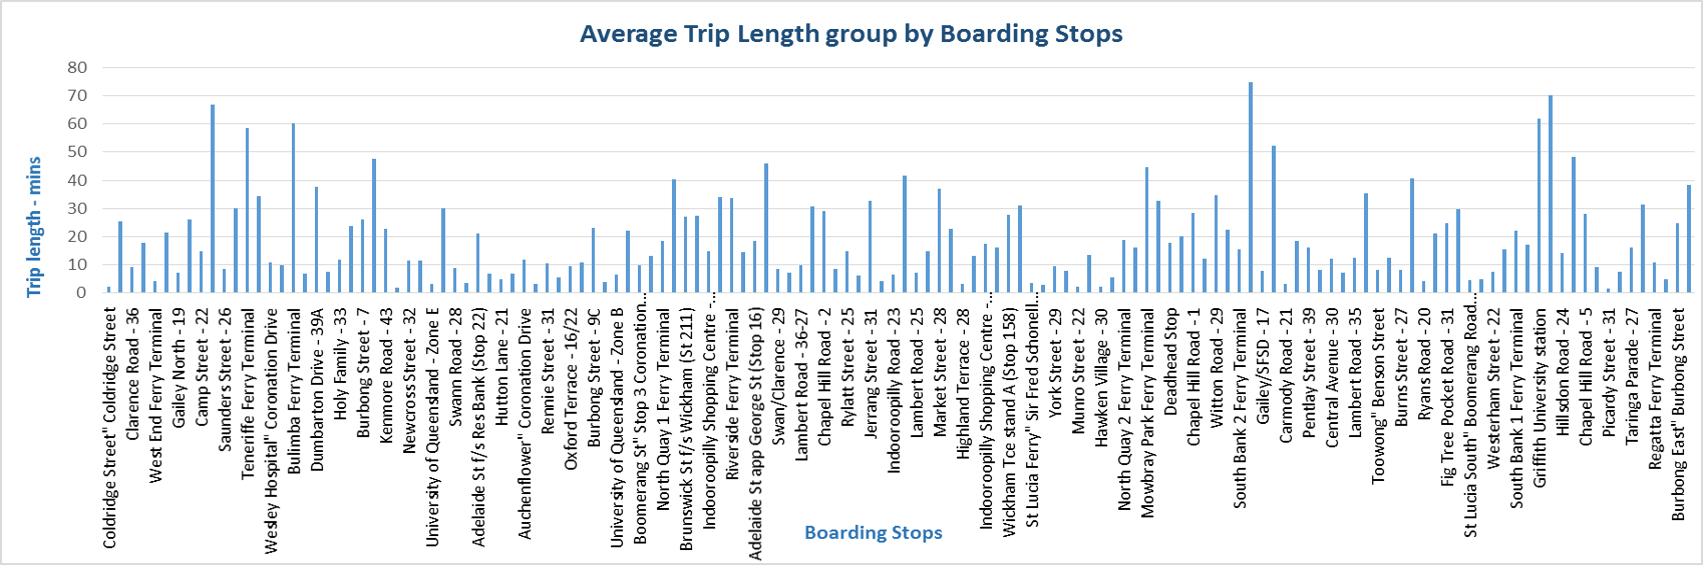
\includegraphics[width=\textwidth]{example.png}
 	\caption{2-Dimensional bar chart visualization generated by query $Q_1$. The x-axis represents the boarding stop, while the y-axis represents the average trip lengths in minutes, towards University of Queensland” stop.}
	\label{fig:q1_vis}
\end{figure}
%
%
%
%
%
%
%
Example \ref{ex:gocard} above suggests that visualizations that portray trend deviations from a reference are potentially remarkable and of high interest.
%

Here, the average trip length grouped by boarding stops (Figure \ref{fig:q1_vis} ) is considered as the top interesting visualization, among other visualizations such as total daily passengers grouped by direction, maximum trip length grouped by boarding stop, and so on.
%
The reason is, it depicts long average trip length in some boarding stops which travels towards UQ that are significantly different from the equivalent average of the trip lengths (equals 17.6 minutes) in the entire dataset. 
%
As listed in Figure \ref{fig:table_gocard_ex}, ferry terminals scored longer trips to UQ than bus stops because ferries often take longer waiting times among stops than buses.
%
%
%
%
%\blue{
\eat{
SeeDB is a data querying and visualization tool that allows analysts to 
manually generate their own visualizations, 
or get data-driven recommendations on demand based on the deviation in data.
%
Specifically, it implements a deviation-based utility metric to identify the most interesting visualizations 
from a large set of potential visualizations. 
%
Then, it posits that a visualization is potentially \emph{interesting} if it 
shows a trend in the subset of data selected by the analyst (i.e., metrics about UQ) 
that deviates from the equivalent trend in the overall dataset. 
%
%}
In our Example \ref{ex:gocard}, the average trip lengths grouped by boarding stops (Figure \ref{fig:gocard_data}) is 
considered as the top interesting visualization produced by SeeDB.
%

However, some bus stops obtained long trips according to the geographical location or the distance such as \emph{Griffith University station}. 
%
%\blue{Abdullah: It is diffcult to know that this view is interesting, so we propose...}
%
%\blue{Add Gap here. Then add list of contribution, then roadmap. Then move to preliminaries and background.}
%\rply{I think we will make the roadmap tomorrow together }
%
}
%
%
%
%
%
%


We summarize our contributions as follows:
%
\begin{itemize}
	\item Proposing a new problem which address the limitation of current visualizations recommendation tools. Particularly, we include budget constraints to automatically
	 recommend top-$K$ interesting visualizations according to an input query within the specified budget.
	 \item Designing an efficient framework called \emph{Realtime Scoring Engine} ($RtSEngine$)
 that limits the exploration of visualizations by assessing priorities of the 
 recommended views according to their deviation utilities and costs.
	\item Proposing efficient algorithms which utilize statistical features of the views such as number 
	of distinct values, selectivity ratios, and data distribution, to early prioritize the views.
	\item Proposing efficient algorithms to approximate the retrieval and computations costs of the generated 
	visualizations and evaluate their estimated costs against their deviation 
	utilities to recommend high accuracy views in the specified budgets.  
	\item Conducting extensive experiments that demonstrate the efficiency and effectiveness of our proposed algorithms on real and synthetic data set.
\end{itemize}
%
This paper is organized as follows: Section \ref{sec:related} describes related works on query visualization. 
%
Then, Section \ref{sec:prelim} provides preliminary details on recommendation of query visualizations and present our problem statement. 
%
Then, we present our framework $RtSEngine$ in Section \ref{sec:method} that contains two main modules: Priority Evaluator and Cost Estimator, which recommend a set of visualizations efficiently within the specified constraints. 
%
Section \ref{sec:expr} shows experiment results for our proposed algorithms on two real datasets. 
%